\documentclass[a4paper, 12pt]{article}
\usepackage[T1]{fontenc}
\usepackage[utf8]{inputenc}
\usepackage[english]{babel}
\usepackage{mathtools}
\usepackage{amsfonts}
\usepackage{amsmath}
\usepackage{mathrsfs}
\usepackage{graphics}
\usepackage{caption}
\usepackage{array}
\usepackage[a4paper,top=2cm,bottom=2cm,left=2cm,right=2cm]{geometry}

\begin{document}
\author{\textsc{Faccin} Dario, 1177736}
\title{\vspace{-2cm} \textsc{Network Analysis and Simulation}}
\vspace{-8ex}
\date{}
\maketitle

\pagenumbering{gobble}

\section*{EXERCISE 1}

\begin{figure}[h!]
	\centering
	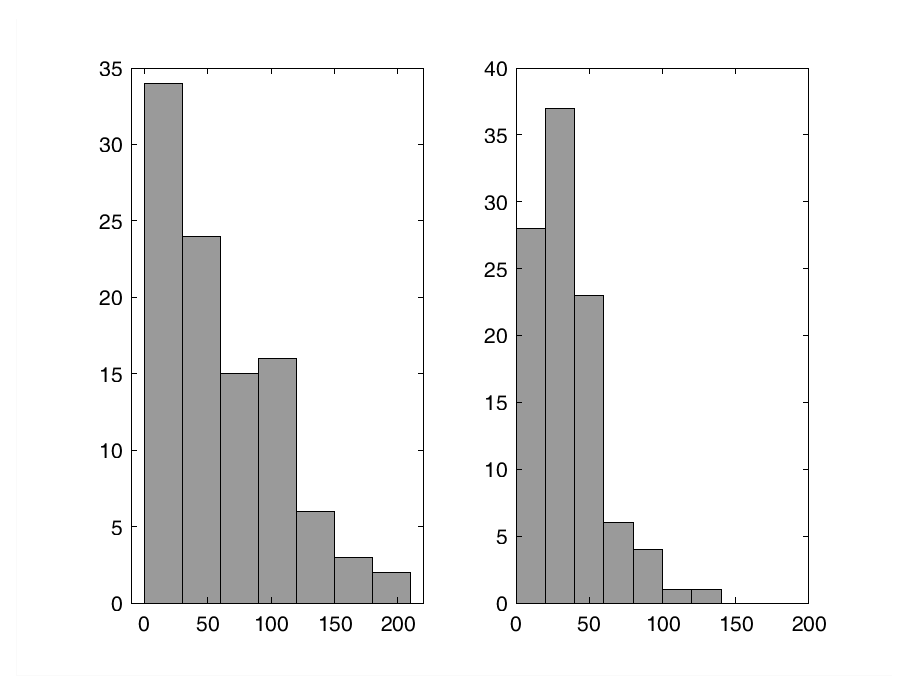
\includegraphics{fig21}
	\caption*{Figura 2.1}
\end{figure} 

\begin{figure}[h!]
	\centering
	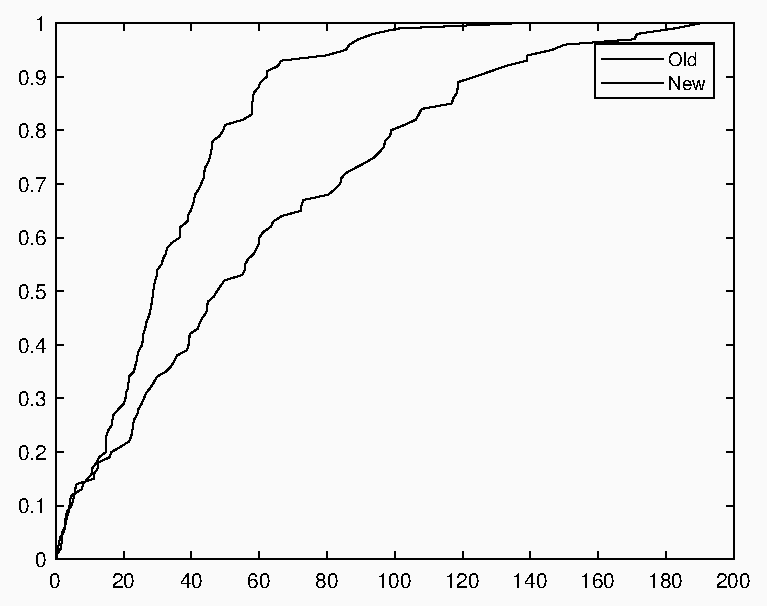
\includegraphics{fig22}
	\caption*{Figura 2.2}
\end{figure} 

\begin{figure}[h!]
	\centering
	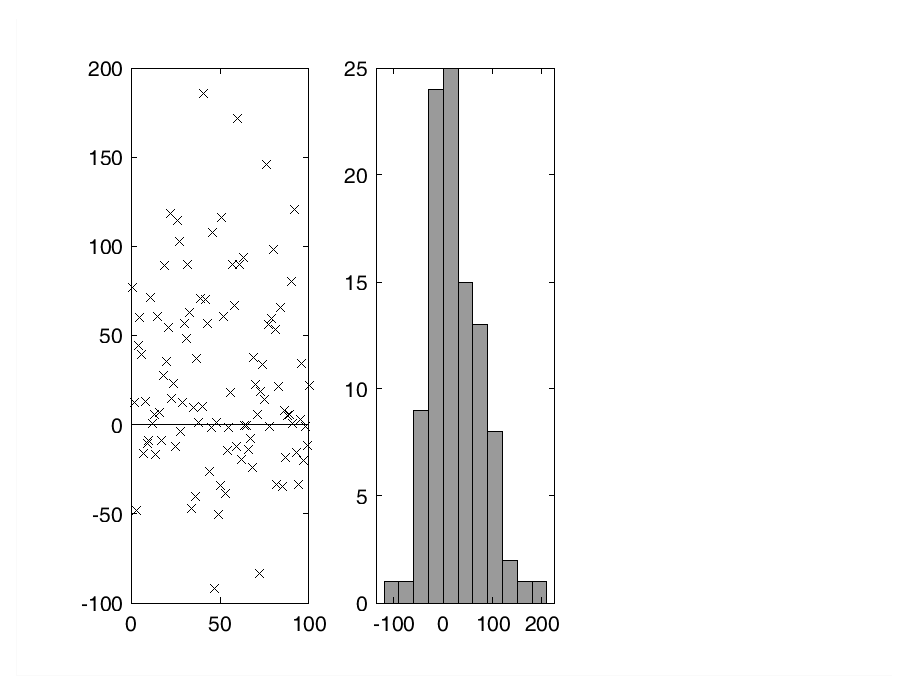
\includegraphics{fig27}
	\caption*{Figura 2.7}
\end{figure} 

\begin{figure}[h!]
	\centering
	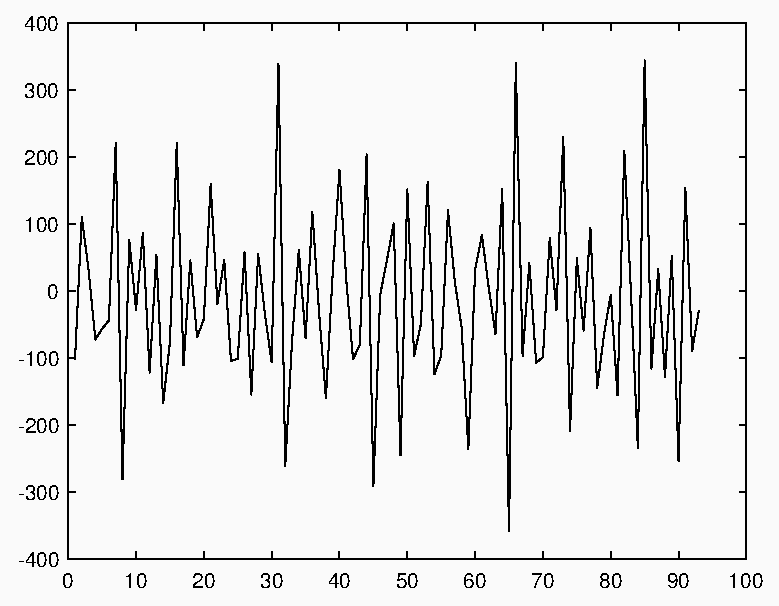
\includegraphics{fig210}
	\caption*{Figura 2.10}
\end{figure} 
\clearpage

\section*{EXERCISE 3}
\begin{itemize}
	\item Confidence interval for 48 i.i.d. U(0,1) random values
	\begin{figure}[h!]
		\centering
		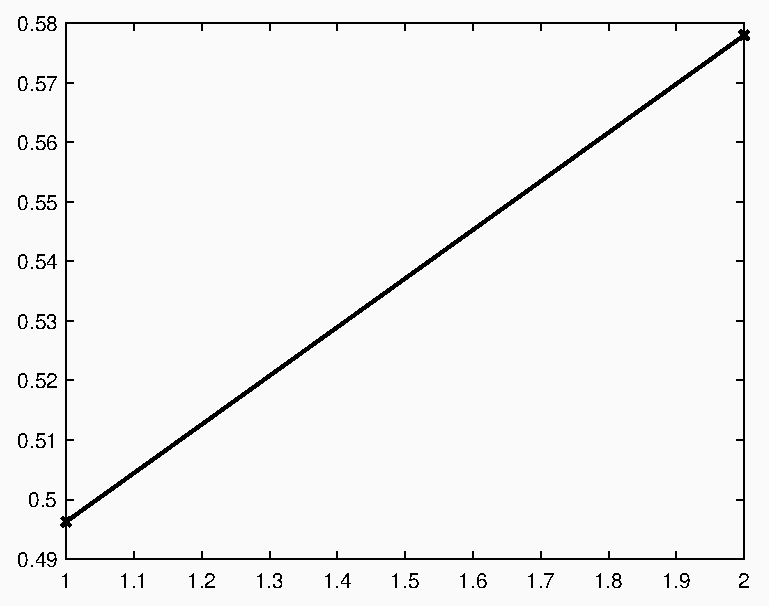
\includegraphics{CIUniformDist}
		\caption*{CI for Uniform Distribuition}
	\end{figure} 

	\item repetition o the experiment for 1000 times 
	\begin{figure}[h!]
		\centering
		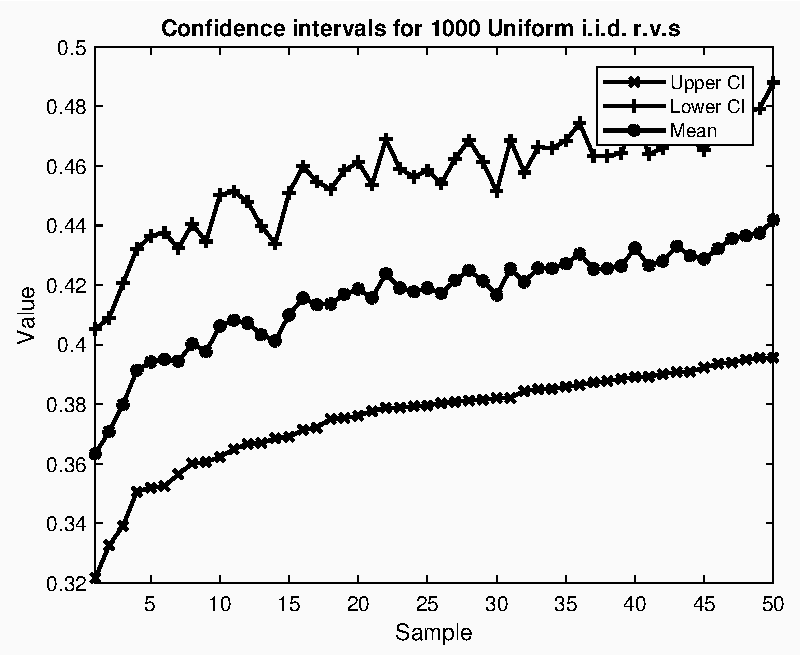
\includegraphics{CIUniformDistFor1000Times}
		\caption*{CI for 1000 times}
	\end{figure} 	
\end{itemize}

\clearpage

\section*{EXERCISE 3}
\setlength\parindent{0pt}
Prove that, for $n$ $U(0,1)$ random variables, we have $ \mathbb{E} \left( U_{(j)} \right) = \frac{j}{n+1}$.\\
\bigbreak
Consider the beta distribution with the following probability density function:\\[5pt]
$f_X(x) =\frac{1}{B(\alpha, \beta)} x^{\alpha -1} (1-x)^{\beta-1} $ defined for $x\in [0,1]$.\\[5pt]
For $ \alpha=1$ and $\beta=1$, it can be shown that the beta distribution coincides with the uniform distribution:
\begin{align*}
	f(x) =\frac{1}{B(\alpha, \beta)} x^{\alpha -1} (1-x)^{\beta-1} & = \frac{\Gamma(\alpha + \beta)}{\Gamma(\alpha) \Gamma(\beta)} x^{\alpha -1} (1-x)^{\beta-1}\\[5pt]
	& = \frac{\Gamma(2)}{\Gamma(1) \Gamma(1)} x^{0} (1-x)^{0}\\[5pt]
	& = \frac{0!}{0!0!} x^{0} (1-x)^{0}\\[5pt]
	& = 1
\end{align*}
Therefore we have $f_X (x) =
\begin{cases}
	1 & x\in [0,1]\\[5pt]
	0 & x\in [0,1]
\end{cases}$, which is the uniform distribution.\\[5pt]
For any positive integer, it holds $\Gamma(m) = (m-1)!$.
\begin{align*}
E(U_{(j)}) &=\frac{n!}{(j-1)!(n-j)!}\int_0^1 x^{j}[1-x]^{n-j}dx \\[5pt]
&= \frac{ \Gamma(n+1)}{\Gamma(j) \Gamma(n-j+1)}\int_0^1 x^{j}[1-x]^{n-j}dx \\
&=\frac{ \Gamma(n+1)}{\Gamma(j) \Gamma(n-j+1)} \cdot \frac{\Gamma(j+1) \Gamma(n-j+1) }{ \Gamma(n+2)} \overbrace{\int_0^1 \frac{ \Gamma(n+2)}{\Gamma(j+1) \Gamma(n-j+1) } x^{j}[1-x]^{n-j}dx}^{=1 \text{ by normalization condition}}\\[5pt]
&= \frac{ \Gamma(n+1)}{\Gamma(j) \Gamma(n-j+1)} \cdot \frac{\Gamma(j+1) \Gamma(n-j+1) }{ \Gamma(n+2)} \\[5pt]
&= \frac{\Gamma(j+1) \Gamma(n+1)}{\Gamma(j) \Gamma(n+2)} = \frac{j}{n+1}.
\end{align*}

\section{EXERCISE 4}
\end{document}